% Use this template to write your solutions to COS 423 problem sets

\documentclass[12pt]{article}
\usepackage[utf8]{inputenc}
\usepackage{amsmath, amsfonts, amsthm, amssymb, algorithm, graphicx, mathtools,xfrac}
\usepackage[noend]{algpseudocode}
\usepackage{fancyhdr, lastpage}
\usepackage[vmargin=1.20in,hmargin=1.25in,centering,letterpaper]{geometry}
\setlength{\headsep}{.50in}
\setlength{\headheight}{15pt}

% Landau notation
\DeclareMathOperator{\BigOm}{\mathcal{O}}
\newcommand{\BigOh}[1]{\BigOm\left({#1}\right)}
\DeclareMathOperator{\BigTm}{\Theta}
\newcommand{\BigTheta}[1]{\BigTm\left({#1}\right)}
\DeclareMathOperator{\BigWm}{\Omega}
\newcommand{\BigOmega}[1]{\BigWm\left({#1}\right)}
\DeclareMathOperator{\LittleOm}{\mathrm{o}}
\newcommand{\LittleOh}[1]{\LittleOm\left({#1}\right)}
\DeclareMathOperator{\LittleWm}{\omega}
\newcommand{\LittleOmega}[1]{\LittleWm\left({#1}\right)}

% argmin and argmax
\newcommand{\argmin}{\operatornamewithlimits{argmin}}
\newcommand{\argmax}{\operatornamewithlimits{argmax}}

\newcommand{\calP}{\mathcal{P}}
\newcommand{\Z}{\mathbb{Z}}
\newcommand{\R}{\mathbb{R}}
\newcommand{\Exp}{\mathbb{E}}
\newcommand{\Q}{\mathbb{Q}}
\newcommand{\sign}{\mathrm{sign\ }}
\newcommand{\abs}{\mathrm{abs\ }}
\newcommand{\eps}{\varepsilon}
\newcommand{\zo}{\{0, 1\}}
\newcommand{\SAT}{\mathit{SAT}}
\renewcommand{\P}{\mathbf{P}}
\newcommand{\NP}{\mathbf{NP}}
\newcommand{\coNP}{\co{NP}}
\newcommand{\co}[1]{\mathbf{co#1}}
\renewcommand{\Pr}{\mathop{\mathrm{Pr}}}

% theorems, lemmas, invariants, etc.
\newtheorem{theorem}{Theorem}
\newtheorem{lemma}[theorem]{Lemma}
\newtheorem{invariant}[theorem]{Invariant}
\newtheorem{corollary}[theorem]{Corollary}
\newtheorem{definition}[theorem]{Definition}
\newtheorem{property}[theorem]{Property}
\newtheorem{proposition}[theorem]{Proposition}

% piecewise functions
\newenvironment{piecewise}{\left\{\begin{array}{l@{,\ }l}}
{\end{array}\right.}

% paired delimiters
\DeclarePairedDelimiter{\ceil}{\lceil}{\rceil}
\DeclarePairedDelimiter{\floor}{\lfloor}{\rfloor}
\DeclarePairedDelimiter{\len}{|}{|}
\DeclarePairedDelimiter{\set}{\{}{\}}

\makeatletter
\@addtoreset{equation}{section}
\makeatother
\renewcommand{\theequation}{\arabic{section}.\arabic{equation}}

% algorithms
\algnewcommand\algorithmicinput{\textbf{INPUT:}}
\algnewcommand\INPUT{\item[\algorithmicinput]}
\algnewcommand\algorithmicoutput{\textbf{OUTPUT:}}
\algnewcommand\OUTPUT{\item[\algorithmicoutput]}


% Formating Macros

\pagestyle{fancy}
\lhead{\sc \hmwkClass $\;\;\cdot \;\;$ \hmwkSemester $\;\;\cdot\;\;$
Problem \hmwkAssignmentNum.\hmwkProblemNum}
%\chead{\sc Problem \hmwkAssignmentNum.\hmwkProblemNum}
%\chead{}
\rhead{\em \hmwkAuthorName\ $($\hmwkAuthorID$)$}
\cfoot{}
\lfoot{}
\rfoot{\sc Page\ \thepage\ of\ \protect\pageref{LastPage}}
\renewcommand\headrulewidth{0.4pt}
\renewcommand\footrulewidth {0.4pt}

\fancypagestyle{fancycollab}
{
    \lfoot{\em Collaborators: \hmwkCollaborators}
}

\fancypagestyle{problemstatement}
{
    \rhead{}
    \lfoot{}
}

%%%%%% Begin document with header and title %%%%%%%%%%%%%%%%%%%%%%%%%

\begin{document}

%%%%%% Header Information %%%%%%%%%%%%%%%%%%%%%%%%%%%%%%%%%%%%%%%%%%%

%%% Shouldn't need to change these
\newcommand{\hmwkClass}{CS 255}
\newcommand{\hmwkSemester}{Spring 2016}

%%% Your name, in standard First Last format
\newcommand{\hmwkAuthorName}{Christian Rentsman}
%%% Your NetID
\newcommand{\hmwkAuthorID}{crentsman}

%%% The problem set number (just the number)
\newcommand{\hmwkAssignmentNum}{5}

%%% The problem number (just the number)
\newcommand{\hmwkProblemNum}{1}

%%% A list of your collaborators' NetIDs, separated by ", ".
%%% You can use a new line ("\\") in the middle to prevent a long
%%% list from overflowing.
\newcommand{\hmwkCollaborators}{}
%%% Sets the collaborator list to appear on the first page
\thispagestyle{fancycollab}

%%%%%%% begin Solution %%%%%%%%%%%%%%%%%%%%%%%%%%%%%%%%%%%%%%%%%%%%%

\section{UVA Results}

\subsection{Problem A: Amalgamated Artichokes}

\begin{center}
    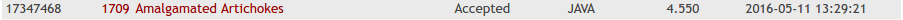
\includegraphics[width=\textwidth]{artichoke_result}
\end{center}

\subsection{Problem C: Catering}

\begin{center}
    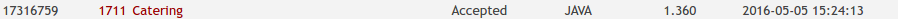
\includegraphics[width=\textwidth]{catering_result}
\end{center}

\subsection{Problem D: Cutting Cheese}

\begin{center}
    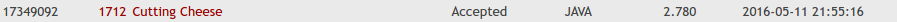
\includegraphics[width=\textwidth]{cheese_result}
\end{center}

\subsection{Problem E: Evolution}

\begin{center}
    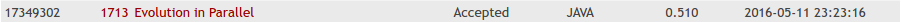
\includegraphics[width=\textwidth]{evolution_result}
\end{center}

\subsection{Problem I: Ship Traffic}

\begin{center}
    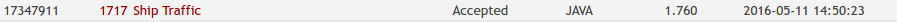
\includegraphics[width=\textwidth]{ships_result}
\end{center}

\newpage

\section{Problem A: Amalgamated Artichokes}

\subsection{Problem Specification}

Fatima Cynara is an analyst at Amalgamated Artichokes (AA). As with
any company, AA has had some very good times as well as some bad ones.
Fatima does trending analysis of the stock prices for AA, and she
wants to determine the largest decline in stock prices over various time
spans. For example, if over a span of time the stock prices were
19, 12, 13, 11, 20 and 14, then the largest decline would be 8
between the first and fourth price. If the last price had been 10
instead of 14, then the largest decline would have been 10 between
the last two prices.

Fatima has done some previous analyses and has found that the
stock price over any period of time can be modelled reasonably
accurately with the following equation:

\begin{center}
    $price(k) = p · (sin(a · k + b) + cos(c · k + d) + 2)$
\end{center}

\noindent where $p, a, b, c$ and $d$ are constants. Fatima would like you to
write a program to determine the largest price decline over a given
sequence of prices. You have to consider the prices only for integer
values of $k$.

\subsection{Mathematical Formulation}

In this problem, given $N$, we have to find the largest decline
in $price(k)$ where $k$ is in $[1, N]$. In other words, we need
to find $i, j$ where $i, j \in [1, N]$ and $i < j$ such that
$price(i) - price(j)$ is the largest difference.

\subsection{Problem Size}

We have an unknown number of test cases, we have to find the largest
decline in prices in under three seconds. However, we know that  $1
\leq p \leq 1000$, $0 \leq a, b, c, d \leq 1000$, and $1 \leq n \leq 10^6$.

\subsection{Solution Description}

To solve this problem, we simply iterate from 1 to $N$, keeping
track of two things: the largest decline we've seen so far, and
the highest price we've seen so far. At every step, we compute
the price and check to see if that price is greater than the
highest price we've seen so far. If it is, we update the highest
price. Then, we check to see if the difference between the
highest price and the current price is greater than the largest
decline we've seen so far. If it is, we update that value as well.
Pseudocode for this process is below:

\begin{algorithm}[H]
\caption{Main runner of our program.}
\begin{algorithmic}
    \Procedure{Main}{}
        \State $in \gets$ new Scanner for system.in
        \While{$in$ has more integers to read}
            \State $p \gets$ next integer from $in$
            \State $a \gets$ next integer from $in$
            \State $b \gets$ next integer from $in$
            \State $c \gets$ next integer from $in$
            \State $d \gets$ next integer from $in$
            \State $n \gets$ next integer from $in$
            \State $maxPrice \gets 0$
            \State $maxDecline \gets 0$
            \For{$i \in [1, n]$}
                \State $currentPrice \gets p * (sin((a * k + b) \% (2\pi)) + cos((c * k + d) \% (2\pi)) + 2)$
                \State $maxPrice \gets$ max between $maxPrice, currentPrice$
                \State $maxDecline \gets$ max between $maxDecline, maxPrice - currentPrice$
            \EndFor
        \EndWhile
    \EndProcedure
\end{algorithmic}
\end{algorithm}

A small note: when we run our price function, we take the sine and
cosine of the remainder of the inner value with $2\pi$. This provides
the same value as it would if we didn't use the remainder (by the
cyclic nature of sine and cosine), but it speeds up the computation.

\subsection{Examples and Test Cases}

Imagine, from some input, we produced this prices from
1 to $N$:

\begin{center}
    19 12 13 11 20 14 10
\end{center}

We would start at 19 and find that to be our highest price seen
so far. Then, until 20, which is our next highest price seen so far
we find the differences in prices to be 7, 6, and then 8. So, right
before 20, our highest price seen so far is 19 and our largest
difference seen so far is 8. Then, we run into 20, and so we update
our highest price seen so far to 20.

From there until the end of the prices, we find the differences
between 20 and the rest to be 6 and then 10. At the 14, we find
the difference to be 6, which is less than our largest decline
seen so far (8), so we don't update it. However, at the 10,
our local decline from 20 is 10, which is greater than our largest
decline seen so far, so we update our largest decline seen so far
to 10. That's the end of input, so we find that our largest
decline overall equals 10.

\newpage

\subsection{Correctness}

\begin{proposition}
    Given N, our algorithm finds the largest decline between
    two points with N.
\end{proposition}

\begin{proof}
    Our algorithm keeps track of the highest price seen so far
    and the largest decline seen so far. We keep track of the
    highest price for a couple of reasons. Say we have three
    nonnegative integers $a, b$ and $c$, such that $a > b$ and
    $c < a, c < b$. Then, we know that $a - c > b - c$. In our
    algorithm, $a, b$ and $c$ represent prices. Thus, if we find
    some low price $c$ that occurs after both $a$ and $b$, the larger
    of the two prices between $a$ and $b$ will have a larger decline.
    Thus, keeping track of the highest price seen so far alongside the
    largest delcine seen so far will lead to the right answer.
\end{proof}

\subsection{Efficiency}

\begin{proposition}
    Given N, our algorithm finds the maximum decline in $O(N)$
    worst case time.
\end{proposition}

\begin{proof}
    Since all we do is iterate from 1 to $N$ and perform a constant
    time operation at each step, our algorithm takes $O(N)$ time
    in the worst case.
\end{proof}

\begin{proposition}
    Given N, our algorithm uses up $O(1)$ space to find the maximum
    decline.
\end{proposition}

\begin{proof}
    Our algorithm takes constant worst case space since the only
    things we ever keep track of are $p, a, b, c, d$, the highest
    price seen so far, and the maximum decline, all of which are
    independent of the problem size.
\end{proof}

\newpage

\section{Problem C: Catering}

\subsection{Problem Specification}

Paul owns a catering company and business is booming. The company has $k$
catering teams, each in charge of one set of catering equipment. Every
week, the company accepts $n$ catering requests for various events.
For every request, they send a catering team with their equipment to the
event location. The team delivers the food, sets up the equipment, and instructs
the host on how to use the equipment and serve the food. After the event, the
host is responsible for returning the equipment back to Paul’s company.

Unfortunately, in some weeks the number of catering teams is less than the number
of requests, so some teams may have to be used for more than one event. In these
cases, the company cannot wait for the host to return the equipment and must keep
the team on-site to move the equipment to another location. The company has an
accurate estimate of the cost to move a set of equipment from any location to any
other location. Given these costs, Paul wants to prepare an Advance Catering Map
to service the requests while minimizing the total moving cost of equipment
(including the cost of the first move), even if that means not using all the
available teams. Paul needs your help to write a program to accomplish this task.
The requests are sorted in ascending order of their event times and they are
chosen in such a way that for any $i < j$, there is enough time to
transport the equipment used in the $i$-th request to the location of the
$j$-th request.

\subsection{Mathematical Formulation}

\subsection{Problem Size}

We are given an unknown amount of test cases that we have to solve in under
three seconds. However, our given variables do have bounds. The number
of teams, $k$, and the number of requests, $n$, are both bounded by
0 and 100, inclusive. The $i$th request (counting from 1) has $n - i + 1$
connections to the requests after it.

\subsection{Solution Description}

To solve this problem, we model the input as a bipartite graph, and
then try to find a minimum cost matching. Therefore, the main parts
of our algorithm are: read in the input and build an adjacency matrix
for a bipartite graph, and then, using that graph and a minimum
cost bipartite matching algorithm with Dijkstra's single source
shortest paths (with an indexed minimum priority queue), find the
minimum cost matching.

The main runner for our program is written below. It is essentially
the algorithm described above.

\begin{algorithm}[H]
\caption{Main runner of our program.}
\begin{algorithmic}
    \Procedure{Main}{}
        \State $in \gets$ new Scanner for system.in
        \While{$in$ has more integers to read}
            \State $n \gets$ next integer from $in$
            \State $k \gets$ next integer from $in$
            \State $g \gets$ \Call{BuildGraphFromInput}{$in, n, k$}
            \State $minCost \gets$ \Call{GetMinCostMatching}{$g, n, k$}
            \State \Call{Print}{$minCost$}
        \EndWhile
    \EndProcedure
\end{algorithmic}
\end{algorithm}

Before we can even solve the problem, we have to build a graph which
represents it. When we call the {\sc BuildGraphFromInput} method,
we read in the input from standard input and we build our bipartite
graph using that data. The nodes on the left part of the bipartite
graph represent preceding locations, and nodes on the right part
of the bipartite graph represent destinations. The algorithm for
building the graph is detailed below:

\begin{algorithm}[H]
\caption{Builds a bipartite graph from the input.}
\begin{algorithmic}
    \Procedure{BuildGraphFromInput}{$in, n, k$}
        \State $numNodes \gets 1 + k + (2 \times n)$
        \State $leftStart \gets 1$
        \State $rightStart \gets k + n$
        \State $g \gets$ new array of size ($numNodes \times numNodes$)
        \State Fill up all indices of $g$ with $\infty$
        \State $teamValues \gets$ new array of size ($numNodes$)
        \\
        \For{$i \in [0, numNodes)$}
            \State $teamValues[i] \gets$ next integer from $in$
        \EndFor
        \For{$u \in [leftStart, k]$}
            \For{$i \in [0, n)$}
                \State $g[u][k + n + i] \gets teamValues[i]$
            \EndFor
        \EndFor
        \For{$u \in [leftStart + k, rightStart)$}
            \For{$v \in [u + n, numNodes - 1)$}
                \State $g[u][v] \gets$ next integer from $in$
            \EndFor
        \EndFor
        \For{$i \in [leftStart, rightStart)$}
            \State $g[0][i] \gets 0$
        \EndFor
        \For{$i \in [rightStart, numNodes - 1)$}
            \State $g[i][numNodes - 1] \gets 0$
        \EndFor
        \\
        \State \Return $g$
    \EndProcedure
\end{algorithmic}
\end{algorithm}

After building our bipartite graph, we simply run a minimum cost
bipartite matching algorithm (our specific implementation utilizes
Dijkstra's Single Source Shortest Paths algorithm with an indexed
minimum priority queue) to find the minimum matching cost. This is
done within the {\sc GetMinCostMatching} method. After doing that,
we just print out the value we found and, thus, the problem is solved.

\subsection{Examples and Test Cases}

To show how our algorithm actually works, we'll run through a quick
example using one of the sample test cases. Say our input is as
follows:

\begin{center}
    3 2 \\
    40 30 40 \\
    50 10 \\
    50
\end{center}

This means that we have three requests ($n = 3$) and two teams ($k = 2$).
We can draw this input as a location graph, showing us the connections
between different locations and the costs to move from one location
to another.

\begin{center}
    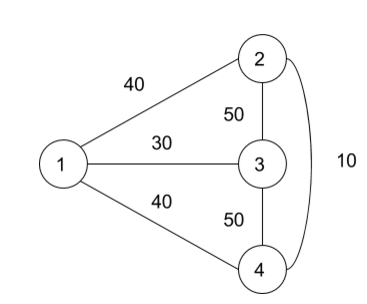
\includegraphics[scale=0.5]{catering1}
\end{center}

However, to actually solve this problem, we need to create a bipartite
graph so we can use the minimum cost bipartite matching algorithm. The
graph and the corresponding adjacency matrix can be found below (vertex
numbers are in parentheses, T means team, and L means location):

\begin{center}
    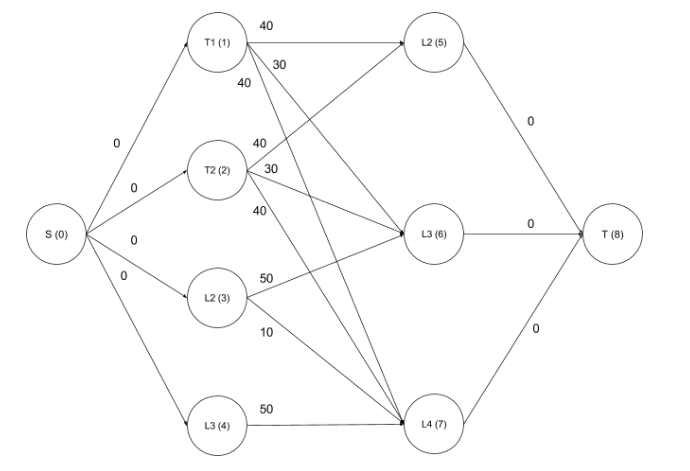
\includegraphics[scale=0.5]{catering_example_graph}
\end{center}

\begin{center}
    \[
        \begin{bmatrix}
            \infty & 0 & 0 & 0 & 0 & \infty & \infty & \infty & \infty \\
            \infty & \infty & \infty & \infty & \infty & 40 & 30 & 40 & \infty \\
            \infty & \infty & \infty & \infty & \infty & 40 & 30 & 40 & \infty \\
            \infty & \infty & \infty & \infty & \infty & \infty & 50 & 10 & \infty \\
            \infty & \infty & \infty & \infty & \infty & \infty & \infty & 50 & \infty \\
            \infty & \infty & \infty & \infty & \infty & \infty & \infty & \infty & 0 \\
            \infty & \infty & \infty & \infty & \infty & \infty & \infty & \infty & 0 \\
            \infty & \infty & \infty & \infty & \infty & \infty & \infty & \infty & 0 \\
            \infty & \infty & \infty & \infty & \infty & \infty & \infty & \infty & \infty \\
        \end{bmatrix}
    \]
\end{center}

\hfill

When we run the minimum cost bipartite matching algorithm on this adjacency
matrix, we find that the minimum cost is 80. That corresponds to sending
team 1 to location 2 then 4, and sending team 2 to location 3.

\subsection{Correctness}

\begin{lemma}
    The minimum cost bipartite matching algorithm finds the minimum
    cost matching for graphs with only imperfect matchings.
\end{lemma}

\begin{proof}
    We know that the minimum cost bipartite matching algorithm finds
    the minimum cost {\em perfect} matching. However, it does so
    by making sure that at every step the matching at that step
    is the lowest costing one. Furthermore, at every step, the cardinality
    of the matching increases by one. Therefore, the algorithm
    finds the maximum cardinality minimum cost matching even
    for graphs where no perfect matching is possible.
\end{proof}

\begin{proposition}
    By modeling the catering problem as a bipartite graph, by
    running the minimum cost bipartite matching algorithm on it
    we get the minimum cost of servicing each request.
\end{proposition}

\begin{proof}
    In our formulation, we model the catering problem as a
    bipartite graph where the nodes on the left represent
    starting locations and the nodes on the right represent
    ending locations. Therefore, a match between a node on
    the right and a node on the left represents the movement
    of a team from one location to another location. The
    number of nodes on the right side of the graph is equal
    to the number of requests, so the highest number of
    matches we could have is equal to the number of requests,
    representing that each request is serviced. Therefore,
    by running the minimum cost bipartite matching on this
    graph, even though a perfect matching may be impossible,
    we find the minimum cost of servicing all requests (see
    the previous lemma).
\end{proof}

\subsection{Efficiency}

\begin{proposition}
    Given N requests and K teams, our algorithm finds
    the minimum cost of servicing all requests in $O((N^3)
    log(N+K))$ time in the worst case.
\end{proposition}

\begin{proof}
    In our formulation, we have a total of $1 + K + (2 * N)$
    nodes (two for the source and the sink, one for each team,
    one for the last location, and two for all other locations).
    We also know that running Dijkstra's single source shortest
    paths with an indexed minimum priority queue takes $O(ElogV)$
    time in the worst case, where $E$ is the number of edges and
    $V$ is the number of nodes. In our graph, we have the number
    of nodes found above, as well as $O(N+K)$ edges from source
    to the left nodes, $O(N^2)$ edges between the left nodes
    and the right nodes (each location has one less edge than
    the previous, and there are $N$ locations so $N(N+1)/2$),
    and $O(N-1)$ edges from each of the right nodes to the sink.
    Therefore, our Dijkstra's takes $O(N^2 log(N+K))$ time. Then,
    we run Dijkstra's $N$ times to match all requests, so our
    algorithm takes $O(N^3 log(N+K))$ time in the worst case.
\end{proof}

\begin{proposition}
    Given N requests and K teams, our algorithm takes up
    $O((N+K)^2)$ to find the minimum cost of servicing
    all requests.
\end{proposition}

\begin{proof}
    As said before, there are $1 + K + (2 * N)$ nodes in our
    graph, which bounds us to $O(N+K)$ nodes. The big data
    structure we use is an adjacency matrix with $O(N+K)$
    entries for each of the nodes, meaning that its size
    is $O((N+K)^2)$ in the worst case.
\end{proof}

\newpage

\section{Problem D: Cutting Cheese}

\subsection{Problem Specification}

Of course you have all heard of the International Cheese Processing
Company. Their machine for cutting a piece of cheese into slices
of exactly the same thickness is a classic. Recently they produced
a machine able to cut a spherical cheese (such as Edam) into
slices---no, not all of the same thickness, but all of the
same weight! But new challenges lie ahead: cutting Swiss cheese.

Swiss cheese such as Emmentaler has holes in it, and the holes may
have different sizes. A slice with holes contains less cheese and
has a lower weight than a slice without holes. So here is the
challenge: cut a cheese with holes in it into slices of equal weight.

By smart sonar techniques (the same techniques used to scan unborn
babies and oil fields), it is possible to locate the holes in the
cheese up to micrometer precision. For the present problem you may
assume that the holes are perfect spheres. Each uncut block has size
$100 \times 100 \times 100$ where each dimension is measured in millimeters.
Your task is to cut it into $s$ slices of equal weight. The slices
will be 100 mm wide and 100 mm high, and your job is to determine the
thickness of each slice.

\subsection{Mathematical Formulation}

Each block of cheese is $100 \times 100 \times 100$ measured in millimeters.
There will be $n$ holes and $s$ slices to make. Each hole is a sphere.
Each hole also has an $x, y$ and $z$ coordinate, which represents where
the center of the hole is within the block of cheese. Each hole also
has an $r$, which corresponds to the radius of the sphere. No holes
overlap, but they touch, and each hole is fully contained by the block
of cheese (or just touches its border). Each of these figures is
measured in micrometers.

\subsection{Problem Size}

We have an unknown amount of test cases to solve, and three seconds
to solve all of them. We know that $0 \leq n \leq 10000$, $1 \leq s
\leq 100$, and $0 \leq x, y, z \leq 10000$.

\subsection{Solution Description}

To solve this problem, we have two main data structures: the block
of cheese and the holes. The block of cheese containers spheres
which represents the holes it has. To distill our algorithm down
to a couple of basic steps, we first construct the block of cheese
containing all of the holes. Then, we find the actual volume of
the cheese by subtracting the volume of each hole from the total
block's volume. Then, we find the volume each slice needs to have
by subtracting the found volume by the number of slices we need.
Then, we use binary search to find where we make slices such that
each slice is the same volume, leading to each slice taking up the
same weight. We do this for every slice except for the last slice,
which we do outside the loop.

\begin{algorithm}[H]
\caption{Main function for our program.}
\begin{algorithmic}
    \Procedure{Main}{}
    \State $in \gets$ new Scanner for system.in
    \While{$in$ has more more to read}
        \State $numHoles \gets$ next integer from $in$
        \State $numSlices \gets$ next integer from $in$
        \State $block \gets$ new block of cheese
        \State $holes \gets$ read in hole from input
        \\
        \State Add holes to $block$, updating its volume for each hole
        \State Sort holes by bottom point closest to the bottom of block
        \State $sliceVolume \gets$ volume of block divided by $numSlices$
        \State $lastCutEnd \gets 0$
        \\
        \For{$i \in [1, numSlices - 1]$}
            \State $cutHeight \gets$ \Call{NextSlice}{$block, lastCutEnd, sliceVolume$}
            \State $cutWidth \gets cutHeight - lastCutEnd$
            \State \Call{Print}{``\%.9f\textbackslash n'', $cutWidth / 1000.0$}
            \State $lastCutEnd \gets cutHeight$
        \EndFor
        \\
        \State \Call{Print}{``\%.9f\textbackslash n'', $(100000 - lastCutEnd) / 1000.0$}
    \EndWhile
    \EndProcedure
\end{algorithmic}
\end{algorithm}

\begin{algorithm}[H]
\caption{Finds the next slice to cut.}
\begin{algorithmic}
    \Procedure{NextSlice}{$block, start, targetVolume$}
        \State $lo \gets start$
        \State $hi \gets 100000$
        \While{$hi > lo$}
            \State $mid \gets (hi + lo) / 2.0$
            \State $sliceVolume \gets$ \Call{volumeOfSlice}{$block, start, mid$}
            \If{$sliceVolume$ is within 10000 to $targetVolume$}
                \State \Return $mid$
            \ElsIf{$sliceVolume > targetVolume$}
                \State $hi \gets mid$
            \Else
                \State $lo \gets mid$
            \EndIf
        \EndWhile
    \EndProcedure
\end{algorithmic}
\end{algorithm}

\newpage

\begin{algorithm}[H]
\caption{Finds the volume of the block between two points}
\begin{algorithmic}
    \Procedure{NextSlice}{$block, start, end$}
        \State $volume \gets 100000 \times 100000 \times (end - start)$
        \For{each $hole$ within the block}
            \If{$hole$ ends before $start$} {\bf continue} \EndIf
            \If{$hole$ starts after $end$} {\bf break} \EndIf
            \State $volume \gets volume - $ \Call{VolumeBetween}{$hole, start, end$}
        \EndFor
        \State \Return $volume$
    \EndProcedure
\end{algorithmic}
\end{algorithm}

\begin{algorithm}[H]
\caption{Finds the volume of a sphere between two points}
\begin{algorithmic}
    \Procedure{VolumeBetween}{$hole, start, end$}
        \If{Entire hole is within $start$ and $end$}
            \State \Return volume of $hole$
        \ElsIf{Only bottom section of hole is within $start$ and $end$}
            \State \Return volume of bottom section
        \ElsIf{Only top section of hole is within $start$ and $end$}
            \State \Return volume of top section
        \ElsIf{Only middle section of hole is within $start$ and $end$}
            \State \Return volume of $hole -$ volume of top section $-$ volume of bottom section
        \EndIf
    \EndProcedure
\end{algorithmic}
\end{algorithm}

Using the four algorithms above, we can find the proper width of each slice
so that each slice is the same weight. The only thing to note of is the
fact that we break out of the loop in algorithm 6 if the current hole
starts after our range. We do that because we sorted the holes before hand,
and doing so saves us time.

\subsection{Examples and Test Cases}

To show how our algorithm actually works, we will go through
a test case. Imagine our block of cheese had two holes in it,
one positioned at (20000, 10000, 30000), and one positioned at
(75028, 61234, 80000), both with a radius of 10000 (all of
these values are measured in millimeters). Then, we know
the volume of each sphere is $4.19 \times 10^{12}$.

Since our base volume is $10^{15}$, we take away $2 * 4.19 \times
10^{12}$ away from it, reducing our block's volume to $9.9162
\times 10^{14}$. Then, imagine we had to make two slices. This
means that each slice would have to have a volume of $4.9581
\times 10^{14}$.

When we run our binary search, we find that cutting at 50000
micrometers from the bottom of the block of cheese will give
us this volume. Then, our two slices both have a width of
50000 micrometers, or 50 millimeters.

\newpage

\subsection{Correctness}

\begin{invariant}
    We do not care about the x coordinate and y coordinate of
    each hole.
\end{invariant}

\begin{proof}
    We know this is true since we know that each hole does not
    overlap with any other hole. Thus, we can move each hole to
    any $x$ coordinate and any $y$ coordinate and our answer
    would not be affected.
\end{proof}

\begin{proposition}
    Using binary search finds the best spot to cut for another
    slice of the same weight.
\end{proposition}

\begin{proof}
    When we binary search in this algorithm, we know where we
    can start and the target volume. Our starting point is
    determined by the ending height of the last slice made,
    so no slices ever overlap. Then, we set our highest
    point to be the top of the block. If the volume of this
    cut is too large, we lower our cutting point to the midpoint
    between our starting position and the highest point. Then, if
    the volume of this slice is too large, we lower the cutting point
    again (by half). If its too large, we raise by half. Otherwise,
    if we are within 1000000 of the target volume (our error),
    we return the slice. Once we find our slicing point, we update
    the starting point of the next slice to that point. We continue
    this for all slices, thus finding best width to use for each
    slice.
\end{proof}

\subsection{Efficiency}

\begin{proposition}
    Given N holes and M slices, our algorithm takes up
    $O(NlogN + MN)$ time to find the slice widths in the
    worst case time.
\end{proposition}

\begin{proof}
    We have $N$ holes, so the sorting step at the start
    of our algorithm takes $O(NlogN)$ time. Then, we
    perform a binary search for each slice, totaling
    $M$ binary searches. Each binary search takes at
    most 30 iterations (to get under our error value),
    and also takes $O(N)$ time to compute the volume
    of the slice. Therefore, our worst case time is
    $O(NlogN + MN)$ time.
\end{proof}

\begin{proposition}
    Given N holes and M slices, our algorithm takes up
    $O(N)$ space.
\end{proposition}

\begin{proof}
    The only thing we really keep track of is each hole,
    since we output each slice width when we find it. There
    are $N$ holes, so our algorithm takes up $O(N)$ space
    in the worst case.
\end{proof}

\newpage

\section{Problem E: Evolution in Parallel}

\subsection{Problem Specification}

It is 2178, and alien life has been discovered on a distant planet.
There seems to be only one species on the planet and they do not
reproduce as animals on Earth do. Even more amazing, the genetic
makeup of every single organism is identical!

The genetic makeup of each organism is a single sequence of nucleotides.
The nucleotides come in three types, denoted by ‘A’ (Adenine), ‘C’
(Cytosine), and ‘M’ (Muamine). According to one hypothesis, evolution
on this planet occurs when a new nucleotide is inserted somewhere into
the genetic sequence of an existing organism. If this change is
evolutionarily advantageous, then organisms with the new sequence quickly
replace ones with the old sequence.

It was originally thought that the current species evolved this
way from a single, very simple organism with a single-nucleotide
genetic sequence, by way of mutations as described above. However,
fossil evidence suggests that this might  not have been the case.
Right now, the research team you are working with is trying to
validate the concept of ``parallel evolution'' — that there might
actually have been two evolutionary paths evolving in the fashion
described above, and eventually both paths evolved to the single
species present on the planet today. Your task is to verify whether
the parallel evolution hypothesis is consistent with the genetic material
found in the fossil samples gathered by your team.

\subsection{Mathematical Formulation}

We are given $N$ strings and a source string. Our goal is
to find if there exists two evolutionary paths so that we
can reach the source string by two different sequences of
the $N$ strings, where each string is used by only one
sequence.

\subsection{Problem Size}

We have an unknown amount of test cases and three seconds to solve
all of them. We now that $1 \leq N \leq 4000$, and that each
nucleotide sequence is between 1 and 4000 characters long. We
also know that each nucleotide sequence is unique.

\subsection{Solution Description}

To solve this problem, we try to find two unique evolutionary
sequences originating from our source string. To do so,
we will start with our source string and go through our
ancestors from the ancestor with the longest sequence
to the ancestor with the shortest sequence. If we can
use all of the sequences, with each one appearing in only
one path, we know that two evolutionary paths are possible.

We move from the current sequence backwards because a sequence
is an ancestor if it is a $subsequence$ of the current sequence.
Why this is true will be explained later.

Each evolutionary path starts with the current sequence. Then,
we begin to go through our ancestor list. For each ancestor,
we have a couple of possibilites:

\begin{enumerate}
    \item The ancestor can be part of both evolutionary paths.
    \item The ancestor can be part of one evolutionary path.
    \item The ancestor can be part of neither of the evolutionary paths.
\end{enumerate}

\noindent For each of these possibilities, we do a different thing.

For the first possibility, we keep track of ancestors that can
appear in both paths. We first check to see if that list is
empty. If it is, then we add it to the list of common ancestors.
Then, if it isn't, we check to see if the current ancestor can
be ancestor of the previous common ancestor. If it can, we also
add it to the list of common ancestors. Otherwise, we just
add it to one of the evolutionary paths and move on.

In the second possibility, we just add the ancestor to the
respective evolutionary path.

If the third possibility happens, we know that there cannot be
two evolutionary paths, since there is an ancestor that is not
part of either of the two evolutionary paths, so we stop
our search here and conclude that it is impossible.

Pseudocode for this algorithm is included below:

\begin{algorithm}[H]
\caption{Determines if a given ancestor can be part of a given path.}
\begin{algorithmic}
    \Procedure{isPathAncestor}{$path, ancestor$}
        \State $latestPathMember \gets$ latest member of $path$
        \State \Return if $ancestor$ is a subsequence of $latestPathMember$
    \EndProcedure
\end{algorithmic}
\end{algorithm}

\begin{algorithm}[H]
\caption{Determines if we can add a new common ancestor.}
\begin{algorithmic}
    \Procedure{isPathAncestor}{$commonAncestors, ancestor$}
        \State $latestCommon \gets$ latest member of $commonAncestors$
        \State \Return $lastestCommon$ is {\bf null} {\bf or} $ancestor$ is a subsequence of $latestCommon$
    \EndProcedure
\end{algorithmic}
\end{algorithm}

\begin{algorithm}[H]
\caption{Runs our program.}
\begin{algorithmic}
    \Procedure{Main}{}
    \State $in \gets$ new Scanner for system.in
    \While{$in$ has more to read}
        \State $n \gets$ next integer from $in$
        \State $current \gets$ next string from $in$
        \State $ancestors \gets$ read ancestor sequences from $in$
        \State Sort $ancestors$ from longest sequence to shortest
        \\
        \State $pathOne \gets$ new set containing $current$
        \State $pathTwo \gets$ new set containing $current$
        \State $commonAncestors \gets$ new empty set
        \State $impossible \gets$ {\bf false}
        \For{each $ancestor$ within $ancestors$}
            \If{$ancestor$ is ancestor to both {\bf and} can add new common ancestor}
                \State Add $ancestor$ to $commonAncestors$
            \ElsIf{$ancestor$ is an ancestor for $pathOne$}
                \State Add $ancestor$ to $pathOne$
                \State Add all within $commonAncestors$ to $pathTwo$
            \ElsIf{$ancestor$ is an ancestor for $pathTwo$}
                \State Add $ancestor$ to $pathTwo$
                \State Add all within $commonAncestors$ to $pathOne$
            \Else
                \State $impossible \gets$ {\bf true}
                \State {\bf break}
            \EndIf
        \EndFor
        \\
        \If{{\bf} not $impossible$}
            \State Add all within $commonAncestors$ to $pathOne$
            \State Remove $current$ from both paths
            \State Print out size of both paths on the same line
            \State Print out contents of both paths
        \Else
            \State Print out ``impossible''
        \EndIf
    \EndWhile
    \EndProcedure
\end{algorithmic}
\end{algorithm}

\subsection{Examples and Test Cases}

Imagine our source genome was ``ACMA'', and our
other sequences were ``ACM,'' ``ACA,'' and ``AMA.''
Then, we would see that the first genome ``ACM''
can be ancestors to both evolutionary paths, so
we add it to the common path. We also find that
the next genome ``ACA'' is common to both, but
it is not an ancestor to ``ACM'', so we just add
it to the first path, and add ``ACM'' to the second
path.

Then, we move on to the third genome ``AMA.'' We
find that ``AMA'' isn't an ancestor to both ``ACM''
and ``ACA,'' so it isn't an ancestor to both paths,
so we say that its impossible to have 2 evolutionary
paths from these genomes.

\subsection{Correctness}

\begin{lemma}
    A given sequence is an ancestor of another one if it
    is a subsequence of the other one.
\end{lemma}

\begin{proof}
    By the problem specification, the species evolves by
    adding certain characters into its existing sequence,
    without changing the order in which the old sequence
    appears in the new sequence. This, by definition, is
    a subsequence.
\end{proof}

\begin{proposition}
    Given a source string and a set of ancestors, our
    algorithm determines whether or not two evolutionary
    paths exist.
\end{proposition}

\begin{proof}
    If two evolutionary paths exist, each gvien genome
    sequence must be a subsequence of the original sequence.
    If there is a subsequence that {\em isn't} part of
    the original sequence, then there is a sequence
    that cannot turn back into the original sequence,
    and thus a third path exists that that doesn't evolve
    into the original sequence, contradicting the fact
    that there is only one species on the planet.

    If that does not happen, then by the previous lemma,
    if we go through the ancestors from the longest
    ancestor to the shortest ancestor, then each of the
    shorter ancestors are a subsequence of the
    previous ancestor on one of the paths. This is also
    due to the definition of a subsequence.

    The only hard case is when an ancestor can be part
    of both paths. We handle this two ways: either
    we add it to the common ancestor path if it is
    compatible (subsequence), or if we can start
    a new common ancestor path (the current path is empty).
    Once we find an ancestor that isn't common to both
    paths, we add that ancestor to the path its compatible
    with, and add the common ancestors to the other path.
    We can do this since we know that the common path can
    belong to any of the two paths, and if the current
    ancestor isn't common to both paths, it also isn't
    common to the set of common ancestors, so we have
    to add the common ancestors to path that is incompatible
    with the current ancestor to keep the validity of
    both paths.
\end{proof}

\subsection{Efficiency}

\begin{proposition}
    Given N sequences, with the length of the longest
    sequence being M, we find two evolutionary paths,
    if possible, in $O(NlogN + NM)$ time in the worst
    case.
\end{proposition}

\begin{proof}
    It takes us $O(NlogN)$ time to sort the sequences
    from longest to shortest, and for each sequence,
    it takes us $O(M)$ time to check to see if it is
    an ancestor to one of the paths. Thus, our algorithm
    takes $O(NlogN + MN)$ worst case time.
\end{proof}

\begin{proposition}
    Given N sequences, our algorithm takes u $O(N)$
    space in the worst case.
\end{proposition}

\begin{proof}
    We know that each of the $N$ sequences has to
    appear in only one of the paths. We keep track of
    both paths, so we keep track of a maximum of
    $N$ sequences, meaning our worst case space is
    $O(N)$.
\end{proof}

\newpage

\section{Problem I: Ship Traffic}

\subsection{Problem Specification}

Ferries crossing the Strait of Gibraltar from Morocco
to Spain must carefully navigate to avoid the heavy ship
traffic along the strait. Write a program to help ferry
captains find the largest gaps in strait traffic for
a safe crossing.

Your program will use a simple model as follows. The strait
has several parallel shipping lanes in eastwest direction. Ships
run with the same constant speed either eastbound or westbound.
All ships in the same lane run in the same direction. Satellite
data provides the positions of the ships in each lane. The
ships may have different lengths. Ships do not change lanes and
do not change speed for the crossing ferry.

The ferry waits for an appropriate time when there is an adequate
gap in the ship traffic. It then crosses the strait heading northbound
along a north-south line at a constant speed. From the moment a ferry
enters a lane until the moment it leaves the lane, no ship in that lane
may touch the crossing line. Ferries are so small you can neglect their size.
Your task is to find the largest time interval within which the ferry can
safely cross the strait.

\subsection{Mathematical Formulation}

We are given a set of ships, along with their position, speed, lane,
and direction. We are also given the speed of the ferry. We have
to find the largest interval of time the ferry has to cross safely.

\subsection{Problem Size}

There is an unknown amount of test cases, and we have three
seconds to solve all of them. There will always be between 1
and $10^5$ lanes, and the width of each lane will always between
1 and $1000$. Each lane has the same width. Ships in the same
lane travel in same direction.

The speed of the ferry is 1 and 100. The speed of the ships
are also between 1 and 100. Each ship travels at the same speed.
We are also given the earliest start time and the latest start time,
both between 0 and $10^6$.

Finally, we each lane we are given between 0 and $10^5$ ships.
Each ship has a length between 1 and 1000, and also has a starting
position between $-10^6$ and $10^6$.

\subsection{Solution Description}

To solve this problem, we calculate the intervals where the
ferry cannot cross the strait. To do so, we calculate, for each
lane, when the ferry cannot cross. We start with the closest
lane, find where the ferry cannot cross, and then continue
to the next lane. Then, we merge all of those invalid times
together and find the largest stretch of free time, after
sorting the invalid times by starting time.

To find the times when the ferry cannot cross the lane, we
have to look at each ship. We need to know when each ship
begins to block the ferry from crossing (this includes when
the ferry gets hit by the ship during crossing) and when
each ship stops blocking the ferry. If these times are
actually within when the ferry can move, we save the time.

Pseudocode for our algorithm can be found below:

\begin{algorithm}[H]
\caption{Main Runner of our program.}
\begin{algorithmic}
    \Procedure{Main}{}
    \State $in \gets$ new Scanner for system.in
    \While{$in$ has more to read}
        \State $numLanes \gets$ next integer from $in$
        \State $laneWidth \gets$ next integer from $in$
        \State $shipSpeed \gets$ next integer from $in$
        \State $ferrySpeed \gets$ next integer from $in$
        \State $earliestStart \gets$ next integer from $in$
        \State $earliestEnd \gets$ next integer from $in$
        \State $blockedTimes \gets \emptyset$
        \\
        \For{each $lane \in [1, numLanes]$}
            \State $ships \gets$ read in all ship information
            \For{each $ship \in ships$}
                \State $blockStart \gets$ when the ship begins blocking the ferry's path
                \State $blockEnd \gets$ when the ship stop blocking the ferry's path
                \If{the block is within our ferry's travel times}
                    \State add interval from $blockStart$ to $blockEnd$ to $blockedTimes$
                \EndIf
            \EndFor
        \EndFor
        \\
        \State Sort $blockedTimes$ by starting time
        \State Merge overlapping blocked times in $blockedTimes$ together
        \State Print longest gap between $blockedTimes$
    \EndWhile
    \EndProcedure
\end{algorithmic}
\end{algorithm}

\subsection{Examples and Test Cases}

Imagine we had the sample input given to us:

\begin{center}
3 100 5 10 0 100 \\
E 2 100 -300 50 -100 \\
W 3 10 60 50 200 200 400 \\
E 1 100 -300 \\
1 100 5 10 0 20 \\
\end{center}

Then, we would have the following invalid intervals:

\begin{center}
    0.0 to 4.0, \\
    10.0 to 30.0, \\
    20.0 to 40.0, \\
    30.0 to 60.0, \\
    50.0 to 80.0, \\
    60.0 to 100.0
\end{center}

\noindent The largest gap between non-overlapping intervals
is 6.0, so we return 6.0.

\subsection{Correctness}

\begin{proposition}
    Our algorithm finds the longest interval of time where
    the ferry can cross the strait.
\end{proposition}

\begin{proof}
    By finding for each lane and for each ship within the lane
    the time where the ferry cannot cross that lane, we obtain
    a set of invalid times. During all of these times, the ferry
    cannot cross the strait at all, since it would be blocked at
    some point. Thus, if we combine all overlapping times together,
    we get continuous intervals of time where the ferry cannot cross
    the strait. Then, the remaining gaps begin these merged intervals
    represent the times when the ferry can cross the entire straight
    safe all the way. Thus, if we choose the largest out of these
    intervals, we will have the largest time interval during which
    the ferry can cross safely.
\end{proof}

\subsection{Efficiency}

\begin{proposition}
    Given $N$ total ships, our algorithm finds the longest safe interval
    that the ferry can cross in $O(NlogN)$ time.
\end{proposition}

\begin{proof}
    We iterate through each lane, and for each lane we iterate through
    all of the ships in the lane. For each ship, we perform a constant
    time operation. Thus, to go through $N$ ships, we take $O(N)$ time.
    Then, in the worst case, we have $N$ invalid intervals, so it takes
    $O(NlogN)$ time to sort them and another $O(N)$ time to find the
    largest safe interval. Thus, our algorithm takes $O(N)$ time in
    the worst case.
\end{proof}

\begin{proposition}
    Given $N$ total ships, our algorithm takes up $O(N)$ space to
    solve the problem in the worst case.
\end{proposition}

\begin{proof}
    We use a constant number of space for each ship, so that is
    already $O(N)$ space. Then, as said before, in the worst case
    we have $N$ invalid intervals. We use a constant amount of space
    per invalid interval, so that takes up $O(N)$ time as well. Thus,
    in the worst case, our algorithm takes up $O(N)$ space in the
    worst case.
\end{proof}


%%%%%%% end Solution %%%%%%%%%%%%%%%%%%%%%%%%%%%%%%%%%%%%%%%%%%%%%

\end{document}
